\documentclass[letterpaper,12pt]{article}

\usepackage[spanish]{babel}
\usepackage[utf8]{inputenc}
\usepackage{multirow}
\usepackage{tikz}
\usepackage{pgf-pie}
\usepackage{graphicx} % graficos
\usepackage{amsmath}
\usepackage{pgfplots}
\usepackage{textcomp}
\usepackage{siunitx}
\begin{document}
	
	\begin{titlepage}
		
		\begin{center}
			\vspace*{-1in}
			\begin{figure}[htb]
				\begin{center}
					
\includegraphics[width=8cm]{Imagen.jpeg}
				\end{center}
			\end{figure}
		
			\vspace*{0.15in}
			\begin{Large}
				\begin{center}
					\textbf{SISTEMA DE AYUDA AL DIAGNÓSTICO DE
TRASTORNOS DEL DESARROLLO EN
ENTORNOS ESCOLARES}
				\end{center}
			\end{Large}
			\vspace*{0.3in}
			\begin{large}
				ESCUELA SUPERIOR DE INFORMÁTICA\\
			\end{large}
			\vspace*{0.3in}
			\rule{150mm}{0.1mm}\\
			\vspace*{0.6in}
			\begin{large}
				\begin{flushleft}
					{\normalsize Asignatura: Sistemas Basados en el Conocimiento}
				\end{flushleft}
				\begin{flushleft}
					{\normalsize Autores: María Blanco González-Mohino\\} 
				\end{flushleft}
				\begin{flushleft}
					{\normalsize Fecha: 06 de Abril de 2021}
				\end{flushleft}
			\end{large}
		\end{center}
		\end{titlepage}
		\tableofcontents
		\newpage

\section{Aquisición de conocimiento}
	En este archivo solo se muestra la información obtenido a partir de la entrevista 1 hacia un docente del C.E.I.P Albuera (Daimiel), iteración número 1.
	
	\subsection{Recopilación de la primera iteración}
	\begin{flushleft}
	\textbf{Fecha: }13/03/2021 \\
	\textbf{Hora: }12:00 - 13:30 \\
	
	\end{flushleft} 
	\begin{flushleft}
	\textbf{Asistentes: } \\
	\end{flushleft}
	Experta: María de las Cruces González-Mohíno Garzás\\
	Ingeniera: María Blanco González-Mohíno
	
	\begin{flushleft}
	\textbf{Lugar:} Sala de reuniones en el C.E.I.P Albuera (Daimiel)
	\end{flushleft}
	\begin{flushleft}
	\textbf{Modo:} Entrevista no estructurada sin conocimiento previo.
	\end{flushleft}
	\begin{flushleft}
	\textbf{Objetivos de la sesión:}
	\end{flushleft}
	Esta entrevista se enfoca a dos objetivos claramente distinguidos: \\
	
	\begin{flushleft}
	1) Conocer el modo de trabajo seguido en el centro e informar adecuada-
mente de cuales serán los procedimientos a seguir para la correcta realización
del sistema. \\
	2) Extraer el conocimiento necesario para los \textit{trastornos de deficiencia
cognitiva y el trastorno del espectro autista}.
	\end{flushleft}
	
	\textbf{Fuente de conocimiento: }Profesora de infantil	
	Esta elección se ha realizado debida a la amplia experiencia en el centro Albuera (12 años) cumplimentando asi el objetivo número 1, y por la amplia
experiencia en el trabajo con niños con trastornos, objetivo número 2. \\

\textbf{Planteamiento y resultado de la sesión}
Batería de preguntas y respuestas desde una visión más general a una más
específica: \\
Repaso del proyectó a realizar para la correcta comprensión del mismo,
después, dio comienzo la entrevista: \\
	
	\textbf{*Las respuestas de las preguntas se encuentran resumidas para
evitar la extensión innecesaria del documento. Se encuentran
incluidas las partes más relevantes que aportan datos
significativos.} \\

\textit{1.- Primero me gustaría hablar un poco sobre su trabajo, sobre el modo de evaluación empleado a niños entre 3 y 5 años para la deteccion de algún
trastorno en su centro, ¿usa algún tipo de escala de evaluación, o
simplemente emplea observación sistemática?}\\

En infantil todos los profesores del centro utilizan escalas de observación
aprobadas por el inspector. Primero evalúan el sistema sensorial (3 años),
fundamentalmente la vista y el oído para encontrar niños con problemas
morfológicos, como el mal enfoque visual, niños daltónicos, etc. El oído es
fundamental para detectar un trastorno de deficit de atención mediante el
tiempo que ellos prestan atención.\\

\textit{2.- En cuanto a esto último, ¿cuánto tiempo cree que es el necesario para porder decir que el niño sufre un trastorno de deficit de atención?}\\

A edades tempranas es más difícil de determinar, un niño con déficit de
atención no permanece sentado.\\

\textit{3.- Para entrar un poco más en materia y relativo a estas edades, tengo entendido que has trabajado con niños con autismo e incluso derivado por
creer que un niño lo tenía y al contrario, hablamos de un caso en el que un
psiquiatra certificó un trastorno autista de libro en un niño y pensaste que
ese niño no era autista, ¿podría exponer el caso?}\\

El niño no centraba la mirada, típico rasgo de niño autista, pero leía a edades muy tempranas aunque solamente emitía las vocales con la entonación de la palabra, el niño también asociaba los elementos leídos a objetos materiales
y entendía la mayoría de cosas que se le decían, a parte de esto el niño era
empático con sus compañeros. No tenía la atracción por el vacío típica de
personas con este trastorno.\\

\textit{4.- Tengo entendido que la etapa gráfica de los niños también es muy
importante a la hora de detectar algo tipo de trastorno, ¿por qué?} \\

Es cierto, también se puede identificar un niño sobredotado. Los niños
borderline suelen quedarse atrasados en algunas etapas gráficas. \\

\textit{5.- Esto esta ligado a las etapas de comprensión y expresión del niño?} \\
Se puede dar en algunos casos, los niños con algún retraso podrían que-
darse atrás en estas etapas. Se les da información corta y concisa. Si el niño
no es capaz de retener información podría ser comportamiento de alguna
deficiencia cognitiva o déficit de atención. \\

\textit{6.- Si un niño no presenta un juego simbólico, a edades en las que sus
compañeros lo han alcanzado, ¿podría presentar ese niño algún trastorno?} \\

Si, en la psicología evolutiva en la fase de 3 a 6 años se tiene que dar un
juego simbólico, se emplea la técnica del juego en paralelo en niños de 3 años, de esta edad hasta los 6 si no pasan a la fase de juego simbólico podríamos estar hablando de un niño con trastorno autista ya que estos no presentan este tipo de juego. \\

\textit{7.- Vamos a cambiar un poco la linea a la deficiencia cognitiva y el retraso madurativo, ¿utilizais alguna técnica para marcar la linea entre una y otra?} \\

Se le tiene que dar un margen de evolución al niño para que sea capaz
de llegar a los diferentes niveles que ha de alcanzar en la etapa de infantil, si el niño no alcanza los niveles cuando sus compañeros están muy avanzados
podríamos estar hablando de un deficiencia cognitiva, en este caso se emplean
una serie de test, por el contrario, si el niño avanza favorablemente, aunque
vaya más lento que sus compañeros podríamos estar hablando de un retraso
psicoevolutivo.
Aún así se hace un test en la edad de los 5 años. \\

\textit{8.- ¿Cómo detectaría a un borderline estando segura que no tiene un retraso psicoevolutivo?} \\

Mediante test de inteligencia. Hay diferentes factores que influyen, en
general un borderline no es capaz de jugar con sus compañeros, ya que no
entiende las reglas del juego. Por su edad cronológica en relación a la etapa
en la que se encuentra no son capaces de adquirir los contenidos relacionados
a esa edad, si hay esta serie de comportamientos se le pasa el test, aunque
también pueden ser problemas de memoria o de inteligencia. En las etapas
gráficas no suelen llegar a la etapa del renacuajo y no hay conservación de la
materia en el niño. \\

\textit{9.- ¿Cuáles son los factores que te hacen tomar la determinación de
informar a la psicóloga del centro de que un niño tiene una deficiencia
cognitiva más grave?} \\

Hay numerosos factores, el niño no es capaz de imitar, tiene un lenguaje
muy básico, cuando un niño al finalizar infantil tiene un promedio de 2000
palabras en su vocabulario, no empatiza, no controla sus emociones, su desplazamiento no es normal.
Se ve alterado todo, desde su motricidad gruesa. Algunos no son capaces
de comer solos, retener varias ordenes.
En cambio los borderlines no suelen resolver problemas sencillos, pero su
motricidad gruesa no se ve muy afectada, también suelen presentar ecolalia. \\

\textit{10.- Ha hablado de una serie de niveles que los niños han de alcanzar,
quién marca y como están marcados estos niveles y lo que se ha de
conseguir en cada uno de ellos?} \\

El sistema educativo español está basado en las etapas de Vygotsky y
Piaget. Hay tres posibles factores: el niño lo consigue, no lo consigue y está
en proceso. \\

\textit{11.- Hemos hablado del trastorno autista, deficiencias cognitivas y
borderlines, ¿podría englobarlo en trastornos más globáles?} \\

\begin{flushleft}
Deficiencia cognitiva - Trastorno mental.\\
Trastorno del espectro autista - Trastorno neurobiológico.\\
Borderline - Afección mental.\\
\end{flushleft}

\textbf{Plan de análisis} \\
\begin{itemize}
    \item Asociación de comportamientos con sus respectivos trastornos
    \item Identificación de términos de la entrevista
    \item Generación de glosario
\end{itemize}
Se van a tratar de delimitar los términos provenientes de:\\
- Trastornos neurobiológicos.\\
- Trastornos mentales.\\
- Afecciones mentales.\\
Trataremos de delimitar los comportamientos asociados a esta
recopilación de trastornos a gran escala para poder delimitar los
comportamientos de cara a siguientes entrevistas. \\
\textbf{Resultados del análisis} \\
\textit{\textbf{• Identificación de las acciones del profesorado}}
\begin{flushleft}
Documentación de comportamientos del niño en escalas de observación. \\
Observación sistemática del niño. \\
Derivación por parte del profesorado a la psicóloga con un diagnóstico. \\
\end{flushleft}
\textit{\textbf{• Asociación de comportamientos con sus respectivos trastornos}}

Trastorno neurobiológicos: \\
- Focalización. \\
- Atracción por el vacío. \\
- Juego simbólico. \\
- Percepción de emociones. \\
- Empatía. \\
--------------------------------------------------------------------- \\
Trastorno mental: \\
- Comprensión. \\
- Juego simbólico. \\
- Adquisición de conocimiento. \\
- Etapa del renacuajo. \\
- Retención de información. \\
- Imitación. \\
- Palabras promedio. \\
- Motricidad gruesa alterada. \\
--------------------------------------------------------------------- \\
Afección mental: \\
- Resolución de problemas sencillos.\\
- Motricidad gruesa.\\
- Ecolalia.\\
- Percepción de emociones.\\

\begin{flushleft}
\textbf{Comentarios} \\
Se han encontrado muy similares los comportamientos realizados por niños
con diferentes trastornos, en la siguiente entrevista se han de concretar los
diferentes comportamientos que marcan la diferencia entre trastornos.\\
\end{flushleft}


\subsection{Recopilación de la segunda iteración}
\begin{flushleft}
En esta iteración se realizó un cuestionario a 20 profesores del CEIP Albuera y CEIP Calatrava, Daimiel, Ciudad Real. La encuesta fue totalmente anonima y vía online debido al COVID-19. 

\end{flushleft}
\begin{flushleft}
Esta encuesta estaba enfocada a concretar algunos datos de la entrevista anterior y a extraer conocimientos del trastorno TDAH. 
\end{flushleft}
\begin{flushleft}

Se realizaron diferentes secciones de preguntas:
\end{flushleft}
\begin{itemize}
\item Sobre entrevista a experto anterior
\item Sobre TDAH
\item Experiencias personales
\end{itemize} 
\newpage
\begin{flushleft}
\textbf{Cuestionario y respuestas:} \\
\textbf{Sobre entrevista anterior:} \\
\textit{1.- ¿Qué entiende con el término 'borderline'?}\\
\end{flushleft}
\begin{center}
\begin{tikzpicture}
\pie{10.5/Respuesta 2,
    78.9/Respuesta 1,
    5.3/Respuesta 3,
    5.3/Respuesta 4}
\end{tikzpicture} \\
\end{center}
\begin{itemize}
\item \emph{Respuesta 1}: Término utilizado por los expertos parade finir a un niño próximo a la deficiencia. \\
\item \emph{Respuesta 2}: El trastorno borderline se caracterizapor la inestabilidad en los estados deánimo, comportamiento y relacionesinterpersonales de quien lo padece.\\
\item \emph{Respuesta 3}: No lo conocia. \\
\item \emph{Respuesta 4}: Alumnos con una discapacidad intelectual límite. \\
\end{itemize}

\newpage
\begin{flushleft}
\textit{2.- ¿Diría que un niño que presenta discapacidad cognitiva desarrolla empatía?}\\
\end{flushleft}
\begin{center}
 \begin{tikzpicture}
\pie{94.7/Si,
    5.3/No}

\end{tikzpicture}
\end{center}

\begin{flushleft}
\textit{3.- Señala los comportamientos que opina que un niño con deficiencia cognitiva presenta}\\
\end{flushleft}
Todas las respuestas señaladas:

\begin{itemize}
\item No comprende órdenes a los 4 años
\item No presenta juego simbólico al terminar infantil
\item No adquiere conocimientos asociados a su edad cronológica
\item Estancado en la etapa del renacuajo (Etapa encontrada dentro de la etapa gráfica preesquemática)
\item No retiene información
\item No imita
\item Vocabulario reducido
\item Motricidad gruesa alterada
\item Un profesor escribió: ``Todo lo anterior''
\end{itemize}

\begin{flushleft}
\textbf{Sobre TDAH:}
\end{flushleft}
\textit{4.- ``Un niño con déficit de atención (TDAH), por lo general, presenta una conducta hiperactiva o impulsiva'' Responda si cree verdadera o falsa esta afirmación}\\

\begin{center}
 \begin{tikzpicture}
\pie{63.2/Verdadera,
    36.8/Falsa}

\end{tikzpicture}
\end{center}
\textit{5.- En su centro, si un niño presenta TDAH, ¿son capaces de dividir el tipo de déficit de atención que el niño presenta?}\\

\begin{center}
 \begin{tikzpicture}
\pie{72.2/Si,
    27.8/No}

\end{tikzpicture}
\end{center}
\textit{6.- Si su respuesta anterior fue VERDADERA conteste la siguiente pregunta: Indique en que subtipos de TDAH se divide este trastorno en su centro}\\

\begin{tikzpicture}
\begin{axis}[
xbar, xmin=0,
width=12cm, height=6cm, enlarge y limits=0.2,
xlabel={Profesores que han respondido},
symbolic y coords={Falta de atención predominante, Conducta hiperactiva/impulsiva, Combinado},
nodes near coords, nodes near coords align={horizontal},
]
\addplot coordinates {(6,Falta de atención predominante) 
(4,Conducta hiperactiva/impulsiva)
(11,Combinado)};
\end{axis}
\end{tikzpicture}
\newpage
\begin{flushleft}
\textbf{Sobre experiencias personales:}\\
\end{flushleft}
\textit{7.- Cuando ha tenido a un niño con algún tipo de trastorno, ¿Cómo lo ha identificado? Nombra el tipo de trastorno y los diferentes comportamientos seguidos por el niño, puede tener tantos ejemplos como quiera.}

\begin{flushleft}
Respuestas que respondían a la pregunta:\\
\end{flushleft}

\begin{flushleft}
\emph{Primer profesor a responder: }\\
``Dentro del espectro autista es la falta de interacción  con su entorno .
Su mirada perdida, aleteo, balanceos corporales y la necesidad de seguir unas rutinas diarias que si se alteran producen en estos niños una reacción desproporcionada y negativa. Si alteras el orden de sus rutinas pueden tener rabietas algunas veces muy intensas.
En los niños con retraso cognitivo es su falta de simbolismo que repercute tanto en su lenguaje ,comprensivo y expresivo, como en su capacidad para resolver problemas de su entorno cotidiano( subirse a una silla para alcanzar algo) , en su lógica-matemática, en sus producciones plásticas, en su motricidad gruesa y fina.
Poseen una memoria muy limitada tanto en el corto como en el medio y largo plazo
No presenta interés ni curiosidad por nada , resulta muy difícil motivarles'' \\
\end{flushleft}

\begin{flushleft}
\emph{Segundo profesor a responder: }\\
``Déficit de atención , llamadas constantes de atención , dificultad para relacionarse, escasas habilidades sociales , escasa interacción con los demás, hábitos muy mecánicos , aleteo de manos , balanceo sobre sí mismos''
\end{flushleft}

\begin{flushleft}
\emph{Tercer profesor a responder: }\\
``Tea, falta de interacción conjunta, comportamientos restringidos, no flexibilidad cognitiva''
\end{flushleft}

\begin{flushleft}
\emph{Cuarto profesor a responder: }\\
``Lo he identificado al comprobar una actividad distinta al resto de niños de su edad. TDAH: falta de atención, impulsividad no controlada, trabajos sin terminar y con graves errores, etc.''
\end{flushleft}

\begin{flushleft}
\emph{Quinto profesor a responder: }\\
``TDH, incapacidad para concentrarse, impulsividad o distracción''
\end{flushleft}

\begin{flushleft}
\emph{Sexto profesor a responder: }\\
``Trastorno cognitivo grave \\
Los comportamientos: lenguaje casi inexistente, incapacidad casi total de razonamiento, incapacidad casi total para aprender. Nula capacidad de relación social, dificultades motrices importantes. Afectación importante del plano motor,lingüístico, social, afectivo y cognitivo''
\end{flushleft}
\textit{8.- ¿Qué trastorno opina que es el más difícil de identificar desde el punto de vista docente?}\\

\begin{flushleft}
Respuestas recogidas:
\end{flushleft}

\begin{itemize}
\item Trastorno cognitivo: 1 profesor
\item Dislexia: 1 profesor
\item TLP: 1 profesor
\item Asperger: 2 profesores
\item TDAH: 4 profesores
\item TEA: 3 profesores\\
\end{itemize}

\begin{flushleft}
\textbf{Análisis de la entrevista}
\end{flushleft}
\begin{flushleft}
Modificaciones y afirmaciones que se deben llevar a cabo sobre la última iteración:
\end{flushleft}
\begin{itemize}
\item Uso del término borderline de manera correcta en relación a las demás iteraciones.
\item Borramos 'empatía' como comportamiento presentado por niños con discapacidad cognitiva.
\item Comportamientos de niños con deficiencia cognitiva correctos.
\end{itemize}

\begin{flushleft}
Comportamientos de niños con TDAH:
\end{flushleft}
\begin{itemize}
\item Conducta impulsiva o hiperactiva.
\end{itemize}

\begin{flushleft}
Es necesario concretar los diferentes niveles de TDAH en siguientes iteraciones.
\end{flushleft}

\begin{flushleft}
Comportamientos a incluir según diferentes experiencias de distintos profesores:
\end{flushleft}

\begin{flushleft}
\textit{TEA:}\\
\end{flushleft}
\begin{itemize}
\item Balbuceo.
\item Falta de interacción con su entorno.
\item Mirada perdida.
\item Aleteos.
\item Balanceos corporales.
\item Necesidad de rutinas diarias con malas reacciones derivadas de la alteración.
\item Sin flexibilidad cognitiva.
\end{itemize}
\begin{flushleft}

\textit{TDAH:}\\
\end{flushleft}
\begin{itemize}
\item Falta de atención.
\item Trabajos sin terminar.
\item Impulsividad no controlada.
\item Errores graves.
\item Incapacidad de concentrarse.

\end{itemize}

\subsection{Recopilación de la tercena iteración}
\begin{flushleft}
	\textbf{Fecha: }23/04/2021 \\
	\textbf{Hora: }17:30 - 19:45 \\
	
	\end{flushleft} 
	\begin{flushleft}
	\textbf{Asistentes: } \\
	\end{flushleft}
	Expertas: María de las Cruces González-Mohíno Garzás\\
			  Psicóloga del centro C.E.I.P Albuera
	Ingeniera: María Blanco González-Mohíno
	
	\begin{flushleft}
	\textbf{Lugar:} Sala de reuniones en el C.E.I.P Albuera (Daimiel)
	\end{flushleft}
	\begin{flushleft}
	\textbf{Modo:} Entrevista estructurada con conocimiento previo.
	\end{flushleft}
	\begin{flushleft}
	\textbf{Objetivos de la sesión:}
	\end{flushleft}
	Profundizar en el trastorno del espectro autista y asegurar los conocimientos obtenidos en anteriores iteraciones: \\
	
	\begin{flushleft}
	1) Profundizar en el trastorno del espectro autista, especialidad de la psicóloga. \\
	2) Asegurar algunos de los comportamientos en diferentes trastornos obtenidos de entrevistas anteriores.
	\end{flushleft}
	
	\textbf{Fuente de conocimiento: }\\
	\begin{itemize}
	\item Profesora de infantil:	Esta elección se ha realizado debido a la amplia experiencia en el campo de la enseñanza. Esta experta también trabajó en un centro de niños con diferentes capacidades intelectuales y trastornos.
	\item Psicóloga del centro: especializada en el trastorno del espectro autista, el cual se llevará a cabo en esta iteración.
	\end{itemize}
	

\textbf{Planteamiento y resultado de la sesión}
Batería de preguntas y respuestas. \\
	
	\textbf{*Las respuestas de las preguntas se encuentran resumidas para
evitar la extensión innecesaria del documento ya que la entrevista puede resultar demasiado larga. Se encuentran incluidas las partes más relevantes que aportan datos
significativos.} \\

\begin{flushleft}
\textbf{SOBRE TEA}
\end{flushleft}
\textit{1.- La manifestación del TEA varía según el momento de vida en el que se encuentra cada persona, pero, ¿podrían concretarse una serie de características comunes del TEA en cada etapa?}\\

No hay dos personas que presenten los mismos comportamientos ante este trastorno. \\
Comportamientos generalizados: meticulosidad, honestidad, sinceridad, atención por detalles, muy lógicos, no presentan prejuicios, buenos en tareas mecánicas y repetitivas, buen seguimiento de rutinas, conocimiento especializado sobre temas de su interes pero estos temas son muy específicos.\\

Para niños a partir de 3 años:
\begin{itemize}
\item Alteración de la comunicación: déficit en el desarrollo del lenguaje, especialmente en la comprensión, escaso uso del lenguaje, pobre respuesta a su nombre, mala comunicación no verbal (no señalar, no aguantar la mirada).

\item Alteraciones sociales: imitación limitada (no aplauden, por ejemplo), ausencia de juegos con juguetes o con otros objetos, no enseña objetos a los demás, no socializan/acercan a niños/as de su edad, no realiza juegos de ficción, no presenta juego simbólico.

\item Alteración de los intereses, actividades y conductas: mal acoplamiento a cambios, pueden presentar hipersensibilidad a los sonidos y al tacto de otras personas, muerden, pegan, agreden a iguales, oposición al adulto. Algo muy significativo: aleteos.
\end{itemize}

\textit{2.- Tengo entendido que las personas con un alto grado de autismo pueden llegar a comunicarse, intuyo que esta comunicación es muy simple, ¿se conoce algún caso de alguien con una perfecta comunicación con un alto grado de autismo?}\\

De momento no, lo normal es que no ocurra, sería raro que ocurriese, normalmente un niño de entre 3-5/6 años con TEA no se comunica si no es para pedir o rechazar, no suele comunicarse para realizar comentarios.  \\

\textit{3.- ¿Cuáles diría que son los principales factores psicomotrices de un niño con TEA, aparte del aleteo?}\\

No mira a la cara o a los ojos sonriendo a la vez.
En general sus movimientos son muy extraños y repetitivos; tiene rabietas y se resiste ante cambios ambientales; también se ríen y lloran sin motivos aparentes.\\

\textit{4.- ¿Presentaría algún tipo de juego el niño a la edad de los 3 años en adelante aunque este fuese no simbólico?}\\

No, el niño de 3 a 5/6 años presentaría juegos repetitivos, ``rituales de ordenación'' en el que ordena o alinea cosas innecesariamente. \\

\textit{5.- ¿Estos niños, presentarían ecolalia?}\\

Sí, no comprenden ni expresan conceptos abstractos, no pueden conversar, hacen preguntas escasas y repetitivas, algunos combinan 2 o 3 palabras y otros repiten estructuras que han escuchado muchas veces ya sean de la radio, TV, sus padres...

\begin{flushleft}
\textbf{SOBRE CONOCIMIENTOS ANTERIORES}
\end{flushleft}
\textit{6.- Sería correcta los siguientes niveles de TDAH: combinado, conducta hiperactiva o impulsiva y falta de atención predominante} \\

Si.\\

\textit{7.- ¿Cuál sería la forma más acertada de llamar al TEA, Trastorno del espectro autista o Trastorno Generalizado del Desarrollo?} \\

TEA, Trastorno del Espectro Autista, antes se encontraba incluido en el Trastorno Generalizado del Desarrollo, hoy día es un trastorno aparte.
%%%%%%%%%%%%%%%%%%%%%%%%%%%%%%%%%%%%%%%%%%%%%%%%%%%%%%%%%%%%%%%%%%%%%%%%%%
%%%%%%%%%%%%%%%%%%%%%%%%%%%%%%%%%%%%%%%%%%%%%%%%%%%%%%%%%%%%%%%%%%%%%%%%%%
%%%%%%%%%%%%%%%%%%%%%%%%%%%%%%%%%%%%%%%%%%%%%%%%%%%%%%%%%%%%%%%%%%%%%%%%%%
%%%%%%%%%%%%%%%%%%%%%%%%%%%%%%%%%%%%%%%%%%%%%%%%%%%%%%%%%%%%%%%%%%%%%%%%%%
\newpage
\section{Conceptualización}
A continuación se mostrarán los términos más revelantes así como las
relaciones entre ellos. En este apartado se incluirá un glosario con conceptos claves, una tabla objeto-atributo-valor en la que se incluirán los distinto valores que un comportamiento puede adoptar. A parte también se incluira el mapa de conocimiento según el razonamiento del experto.
\subsection{Glosario}
\begin{flushleft}
\textbf{\textit{Lista de elementos y definiciones}}

\textit{1 - Etapa gráfica:} se trata de las etapas universales que presentan los niños de diferentes culturas. Estas etapas son: etapa del garabateo (2-4 años), etapa pre esquemática (4-7 años), etapa esquemática (7-9 años), etapa del realismo (9 y 12 años), etapa pseudonaturalista (12-14 años). \\
\textit{2 - Retraso psicoevolutivo: }Segun Piaget, el desarrollo psicoevolutivo son los distintos cambios por el que el niño pasa desde su nacimiento a nivel físico, cognitivo, lingüístico y socio-emocional. \\
\textit{3 - Motricidad gruesa:} Actividades y movimientos que los niños realizan utilizando los grandes grupos musculares, involucrando las extremidades inferiores, superiores y los movimientos de la cabeza. \\
\textit{4 - Ecolalia:} Repetición involuntaria de palabras o frases. \\
\textit{5 - Etapa de renacuajo:} Etapa encontrada dentro de la etapa gráfica preesquemática, en la que el niño es capaz de dibujar un círculo y elementos que salen de este, siendo estos, normalmente, partes del cuerpo. \\
\textit{6 - Borderline:} Termino utilizado por los expertos para definir a un niño próximo a la deficiencia.\\
\textit{7 - Juego simbólico:} Actividad en la que los niños utilizan su capacidad mental para recrear un escenario. Por ejemplo: algunos niños son doctores y otros pacientes.\\
\end{flushleft}
\begin{flushleft}
\textbf{\textit{Relaciones entre elementos}}\\
6 pertenece a 1. (Etapa de renocuajo - Etapa gráfica) \\
2 precedente a 7. (Retraso psicoevolutivo - Juego simbólico)\\
\end{flushleft}

\begin{flushleft}
\textbf{\textit{Trastornos y sus siglas:}}\\
TDAH: Trastorno por Déficit de Atención e Hiperactividad. \\
TEA: Trastorno del Espectro Autista \\
\end{flushleft}

\begin{flushleft}
\textbf{\textit{Elementos no preocupantes}} \\
Si el niño presenta evolución aunque esta sea lenta. (No confundir con
Borderline) \\
\end{flushleft}

\subsection{Diccionario de conceptos}
\subsubsection{Tabla Objeto-Atributo-Valor}
En la tabla objeto-atributo-valor se encuentran recogidos los conceptos
del dominio del sistema, los atributos que los caracterizan y los posibles valores que los atributos pueden tomar.


\begin{flushleft}
\scalebox{0.8}{\begin{tabular}{|p{5.5cm}|p{5.6cm}|p{6.5cm}|}
 \hline 
 Objeto & Atributo & Valor \\ 
 \hline 
 \multirow{19}{*}{El niño presenta} 
  & Focalización & Si/No \\ 
  & Atracción por el vacío & Si/No \\ 
  & Percepción de emociones & Si/No \\ 
  & Empatía & Si/No \\ 
  & Balbuceo & Si/No \\ 
  & Falta de interacción con su entorno & Si/No \\ 
  & Aleteos & Si/No \\ 
  & Balbaceos corporales & Si/No \\ 
  & Mala reacción al cambio de rutina & Si/No \\
  & Uso del lenguaje & Escaso / Normal \\
  & Respuesta a su nombre & Si/No \\
  & Señala & Si/No \\
  & Enseña objetos & Si/No \\
  & Socialización con niños de su edad & Si/No \\
  & Hipersensibilidad a los sonidos o tacto & Si/No \\
  & Muerden/pegan/agreden a otros niños & Si/No \\
  & Oposición al adulto & Si/No \\
 \hline 
 \end{tabular}}
\end{flushleft}
\begin{flushleft}
\scalebox{0.8}{\begin{tabular}{|p{5.5cm}|p{5.6cm}|p{6.5cm}|}
 \hline 
 Objeto & Atributo & Valor \\ 
 \hline 
 \multirow{12}{*}{Comportamiento del niño} & Comprension 4 años & Si/No \\ 
  & Juego simbólico & Si/No \\ 
  & Adquisición de conocimientos por edad cronológica & Si/No \\ 
  & Etapa del renacuajo & Estancado/No estancado \\ 
  & Retención de información & Si/No/Información básica \\ 
  & Imitación & Imita/No imita \\ 
  & Palabras promedio & [0 - 2000] palabras \\
  & Motricidad gruesa & Alterada/No alterada/Algo alterada \\
  & Resolución de problemas sencillos & Dificultad/No dificultad \\ 
  & Ecolalia & Si/No \\ 
  & Emociones irregulares & Si/No \\ 
 & Impulsividad & Controlada / No controlada \\
 & Atención & Atiende normal / Falta de atención \\
 & Trabajos & Terminados sin problema / Trabajos no terminados / Trabajos con 	errores graves \\
 & Concentración & Incapaz de concentrarse / Concentración normal \\
 \hline 
  \end{tabular}}
\end{flushleft}

\newpage
\subsubsection{Mapa de conocimientos}
El mapa de conocimientos nos permite establecer las relaciones entre los
distintos conceptos y la estructura del razonamiento del experto.
En el mapa podemos observar como el experto le realiza pruebas de comportamiento al niño como llamarlo desde atras para comprobar su sistema auditivo, comprobación de la focalización ya mencionada, entre otras. Con esta serie de características el experto realiza una hipótesis, lo llamado ’Diagnóstico heurístico’. A la par de está realización el experto rellena la escala de observación aprobada por el inspector; con estos dos ’diagnósticos’ se procede a la elección para su posterior elevación del caso al psicólogo y padres.

\begin{figure}[h!]
				\begin{center}
					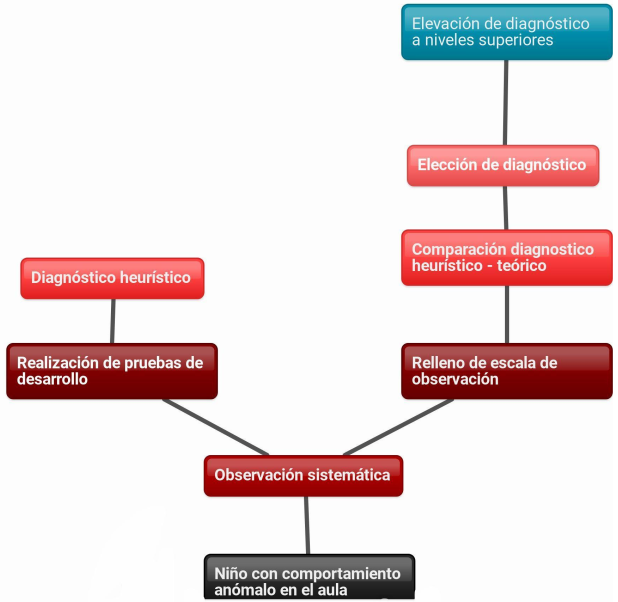
\includegraphics[width=10cm]{Pensar.png}
				\end{center}
			\end{figure}
			
\clearpage
\subsubsection{Ontología}

\section{Representación del conocimiento}
Para la reprensatción del conocimiento de este sistema experto se utiliza
un razonamiento hacia delante basado en reglas, razonamiento basado en
lógica. A continuación se indican las diferentes reglas extraidas mediante las diferentes técnicas de adquisición de conocimiento empleadas: \\

\begin{center}
\begin{tabular}{|c|}
\hline 
\textbf{Regla 1} \\ 
Si el niño no focaliza, — nf \\
siente atracción por el vacío, — av \\
no presenta juego simbólico, — njs \\
sus emociones se encuentran alteradas, — ea \\
y no presenta empatía, — ne \\ 
Entonces el niño presenta un trastorno autista. — autista \\
\hline 
\end{tabular} 
\end{center}
\begin{center}
\begin{tabular}{|c|}
\hline 
 \textbf{Regla 2:} \\
Si el niño no comprende a la edad de 4 años, — nc \\
no presenta juego simbólico, — njs \\
no adquiere los conocimietos correspondientes a esa edad, — nce\\
se encuentra estancado en la etapa del renacuajo, — er\\
no retiene información, — nr \\
no imita, — ni \\
su vocabulario es menor a 2000 palabras, — mp \\
su motricidad gruesa se encuentra alterada, — mg \\
entonces el niño presenta deficiencia cognitiva — deficiencia\\ 
\hline 
\end{tabular} 
\end{center}

\begin{center}
\begin{tabular}{|c|}
\hline 
\textbf{Regla 3:} \\
Si el niño tiene dificultad para resolver problemas sencillos, — nps\\
su motricidad gruesa se encuentra algo alterada, — mg\\
presenta ecolalia, — e\\
sus emociones se encuentras algo alteradas, — ea\\
entonces el niño presenta un trastorno borderline. — borderline \\ 
\hline 
\end{tabular} 
\end{center}

\begin{center}
\begin{tabular}{|c|}
\hline 
\textbf{Regla 4:} \\
Si el niño presenta impulsividad, — \\
falta de atención, — \\
trabajos no terminados o trabajos con errores graves, — \\
es incapaz de concentrarse, — \\
entonces el niño presenta TDAH. — TDAH \\ 
\hline 
\end{tabular} 
\end{center}

Nota: a la derecha de cada comportamiento se encuentra la abreviatura que
se empleará más adelante. \\

Acto seguido podemos ver el ciclo empleado para la obtención de un
diagnóstico así como un ejemplo utilizando las reglas pertenecientes a la correspondiente base de conocimiento: \\

\begin{center}
\begin{tabular}{|p{15cm}|}
\hline 
\textbf{Paso 1:} comprobamos los comportamientos que se presentan y verificamos las posibles reglas que pueden darse,teniendo en cuenta que si hay 3 comportamientos adversos por regla esta no se podrá disparar, si estas condiciones se dan en más de una regla se elegirá la primera por posición. \\
\textbf{Paso 2:} disparamos la regla que tenga más trastornos asociados y borramos el conjunto de reglas posibles.\\
\textbf{Paso 3:} añadimos comportamiento a la memoria de trabajo. \\
\textbf{Paso 4:} Retornamos a paso 1 hasta que los comportamientos expresados solo puedan asociarse a una regla.\\
\textbf{Paso 5:} seleccionar regla y acabar las iteraciones. \\ 
\hline 
\end{tabular} 
\end{center}
\newpage
Ejemplo: \\

\begin{tabular}{|c|p{5.5cm}|c|c|}
\hline 
Iteración & Memoria de trabajo & Reglas posibles & Regla disparada \\ 
\hline 
0 & njs, ea, e & 1,2,3 & 1 \\ 
\hline 
1 & njs, ea, e, mg & 1,2,3 & 1 \\ 
\hline 
2 & njs, ea, e, mg, f & 2,3 & 2 \\ 
\hline 
3 & njs, ea, e, mg, f, mg & 2,3 & 2 \\ 
\hline 
4 & njs, ea, e, mg, f, mg, nps, np & 3 & 3 \\ 
\hline 
5 & njs, ea, e, mg, f, mg, nps, np, \textbf{borderline} & -- & PARAR \\ 
\hline 
\multicolumn{4}{|p{13.3cm}|}{f: focaliza} \\ 
\multicolumn{4}{|p{13.3cm}|}{PARAR: se para cuando no hay conjuntos que suponen un conflicto} \\ 
\hline 
\end{tabular} \\
Se muestra un razonamiento hacia delante (\textit{forward}) basado en reglas.
\end{document}